\chapter{Profile guided optimization}
\label{chap:profile_guided_opti}
The idea is to get profile information during the compilation (or in the
interpreter) of the program, create a profile then use this profile to compile
efficiently the program.
We can see the pipeline using profile here:
\begin{figure}[H]
     \centering
     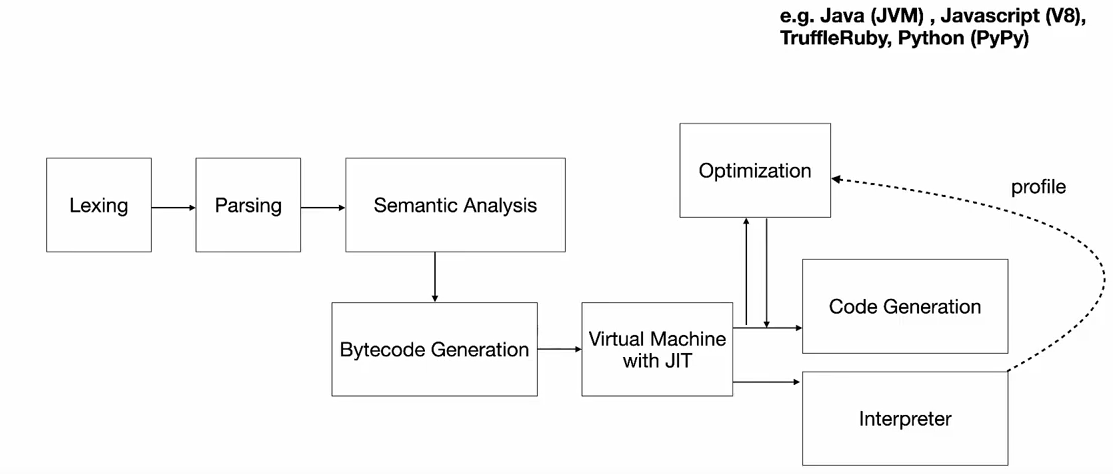
\includegraphics[scale=0.4]{pipeline_profile}
     \caption{Pipeline with profiling}
     \label{fig:pipeline_profiling}
\end{figure}
We can also do ahead of time profile optimization as this pipeline shows:
\begin{figure}[H]
     \centering
     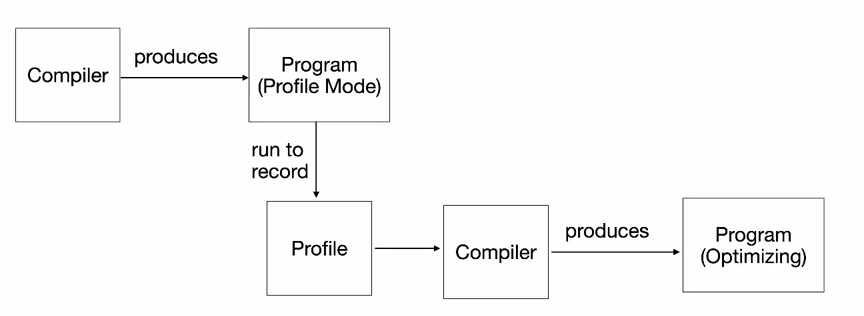
\includegraphics[scale=0.6]{aotpgo}
     \caption{Ahead of time PGO}
     \label{fig:pipeline_pgo}
\end{figure}
The profile helps determine what is common/uncommon and which specialized
version to optimize.
\section{What's profiled?}
The number of calls to each method and the number of loop iteration indeed, if a
loop does millions of iteration we want to optimize it as soon as possible. This
can lead to an interesting point where a function called once but with millions
of iterations can be replacement from it's slow version to the fast one during
its execution (called unstacked replacement or osr). 

Concrete type of Object are also profile (particularity efficient on OOP) it
helps to determine the actual type of virtual calls.

We can also profile the probability of each branch in a if. Values can be also
cached thanks to profile, but in order to do that we must be sure that the value
are stables. Which mean that they won't change, won't change often or small
different values will be used. Sometimes, we start recording, then give up
because to values becomes to broad.

\section{Using the profile}
\subsection{Call and loop counts}
They are used to determine and prioritize which function to compile (if a
function is not called enough, we won't expend resources trying to compile it.)
On the other hand, if we must compile many function, we want to prioritize the
most used one.
\subsection{Concrete types}
Very useful with virtual methods, let's take Java as an example, any non-static,
non-final function is called polymorphic. A polymorphic can be monomorphic,
bimorphic, ..., megamorphic. We can then use \textit{monomorphisation} to
replace all non megamorphic call by its concrete type!

\subsubsection{Monomorphic calls}
\begin{itemize}
    \item Add a check that the test is indeed the type we've always seen so far
    (not necessary if only 1 class if we can't update at runtime. Note that Java
    allow loading classes at runtime.)
    \item Call the call target directly.
\end{itemize}
Doing this gives us two advantages:
\begin{enumerate}
    \item Avoid a potentially expensive lookup
    \item As we know the exact code that will be called, we can inline it.
\end{enumerate}
\subsubsection{Bimorphic calls}
    Replace the lookup by type checks on the known types
    \begin{lstlisting}[language=Java]
        method()
    \end{lstlisting}
    becomes:
    \begin{lstlisting}[language=Java]
        if(type1) method1();
        else if(type2) method2();
        else deopt();
    \end{lstlisting}
    deopt() allow to de-optimize in case new classes are introduce during runtime. 
\subsubsection{Megamorphic calls}
    The more classes we get, the less advantages we have cause we will start to
    pollute the cache. In case of megamorphic we will just give up inlining.
\section{Dynamically typed languages}
If we try to compile these languages we will ends up with a lot of code (need to
check for every type possibility, see slide 8) which is bad for performances:
\begin{itemize}
    \item More code
    \item So more cache pollution
    \item So more cache misses
    \item Besides, we cannot inline must otherwise the cache would end up killed
    by the amount of code. 
    \item The control flow will be huge (does not allow nice and optimizable
    basic blocks)
    \item It would also be very hard to make any assumptions as there is many
    ways to reach some code.
\end{itemize}
\subsection{Specialization}
It's the solution to the problem we just saw. It's like loop unswitching but
used in every operation. It moves conditions to the top and basic blocks in the
middle. Instead of checking type of operation for every block, we do it only
once! Using it with profiles allow to not compiles branches that have been never
seen in practice. 

We can even go further and write our own specialization (like in Truffle).
Thanks to that, we can gives the compiler higher level hints about optimization
that we, programmers, know and for which it is unaware. See example slide 10. On
the example of Truffle on slide 12, we can see that, thanks to profiling we
avoid a lot of specialization compilation as the program see, it's always
integer specialization on the left and string specialization on the right. If we
use numbers, specialization will be compiled out, but if we use variable, we'll
just have guards on the top that does typechecks. If a guard fails, we need to
de-optimize and update the profile, then we can recompile with the new profile!
Another example is given on slide 14.

For now we have only seen specialization for type, but actually we can do it on
anything we can compute! Especially for conditions, where the goal will be to
create fast path for simple cases and compile complex one only if we really need
them (remember that adding compiled code is bad as it bloat cache). These kind
of specialization can be use for empty dictionaries/arrays as the logic is much
more simpler in that cases. String encoding or field structures can also be
cached.

We can also cache values that are expensive to compute. Often these are values
that are computed during runtime (method lookup) and not user-defined. In
Truffle these caches are per-specialization. Note the specialization condition
may depend on the cached value.